\section[Руководство пользователя]{РУКОВОДСТВО ПОЛЬЗОВАТЕЛЯ}
\label{sec:user_manual}

\subsection{Установка приложения}

Приложение может быть установлено только на компьютер с установленной
операционной системой OS X и активным подключением к интернету.

Открыв магазин приложений, нужно ввести в строку поиска название
приложения~(StatusBarApp) и дождаться результатов поисковой операции.
После выбора пользователем необходимого приложение, начнётся процесс установки.

Когда процесс установки закончится, пользователь сможет найти установленное
приложение в Launchpad. Пример расположения утсановленного приложения
в Launchpad изображен на рисунке~\ref{pic:launchpad}.

\begin{figure}[h!]
  \centering
  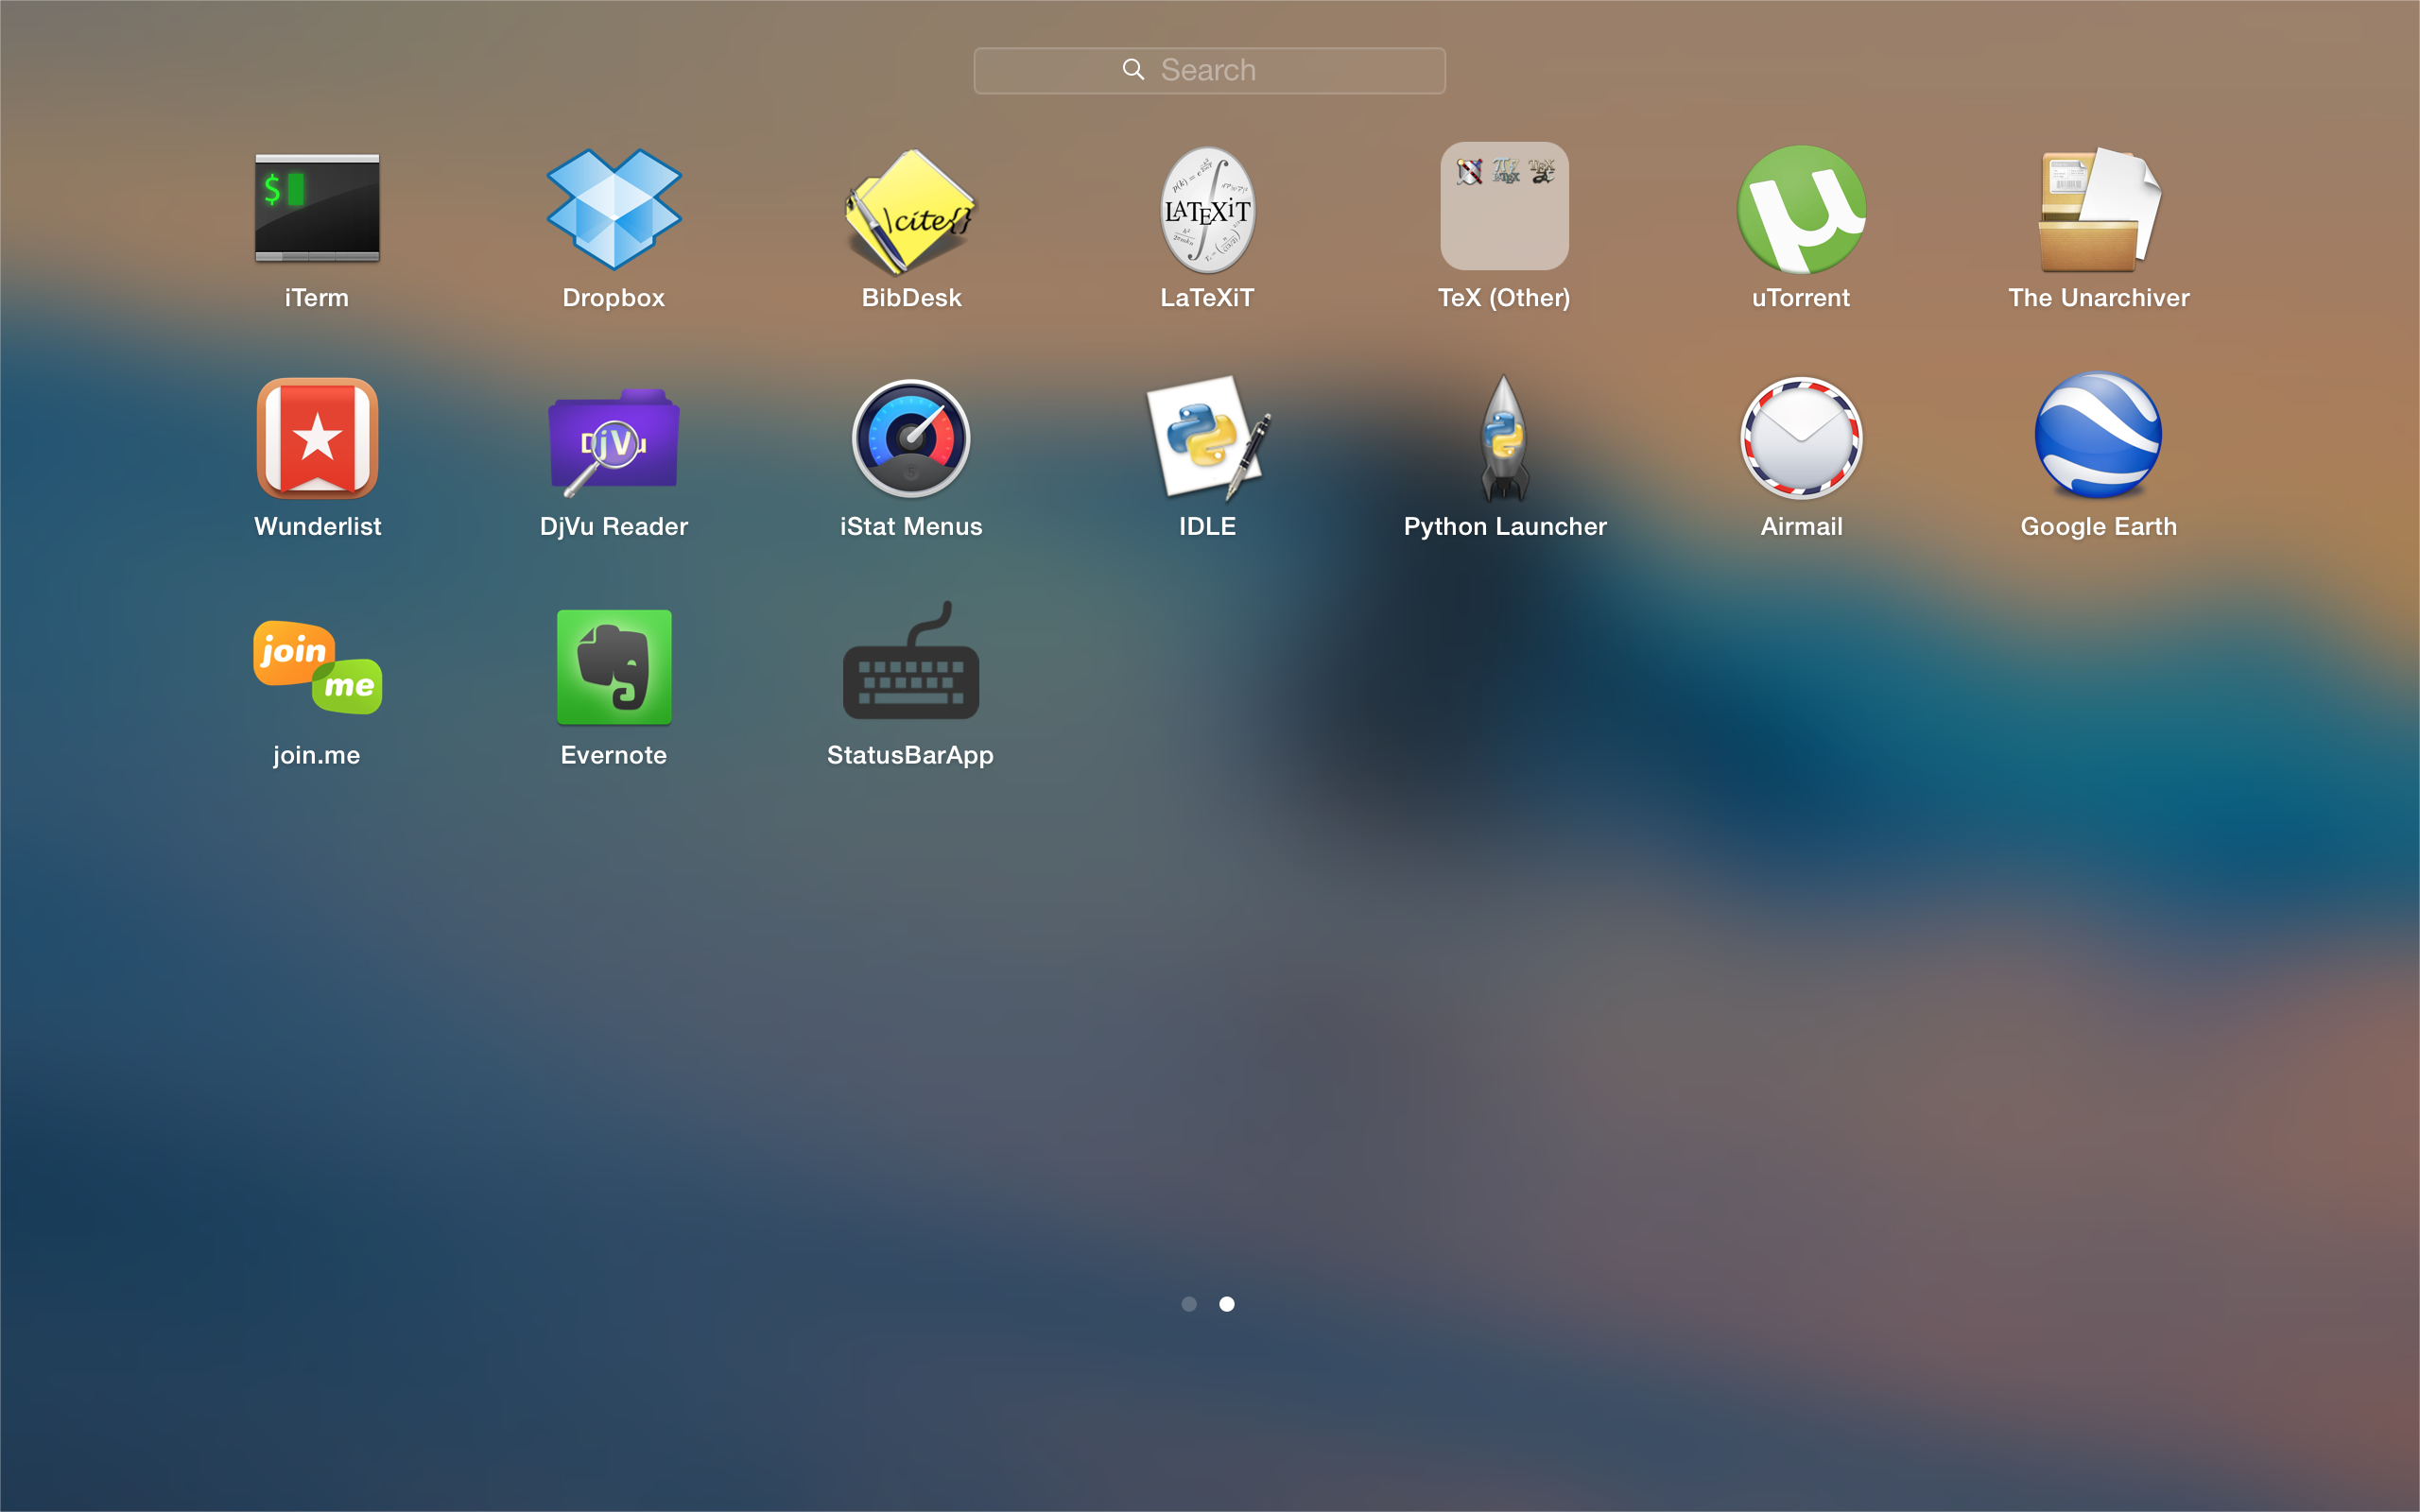
\includegraphics[width=150mm]{pic/launchpad.png}
  \caption{Пример расположения приложения в Launchpad}
  \label{pic:launchpad}
\end{figure}

\newpage

\subsection{Использование приложения}

Сразу после запуска приложение скрывает все активные окна. Факт работы
приложения можно подтвердить с помощью появившейся иконки в статус баре.
По нажатию на иконку появляется меню с доступными функциями, изображенное
на рисунке~\ref{pic:statusbar}. При выборе пункта меню <<Показать лог>>
открывается журнал с записями о нажатых клавишах, представленный
на рисунке~\ref{pic:log_window_in_work}.

\begin{figure}[h!]
  \centering
  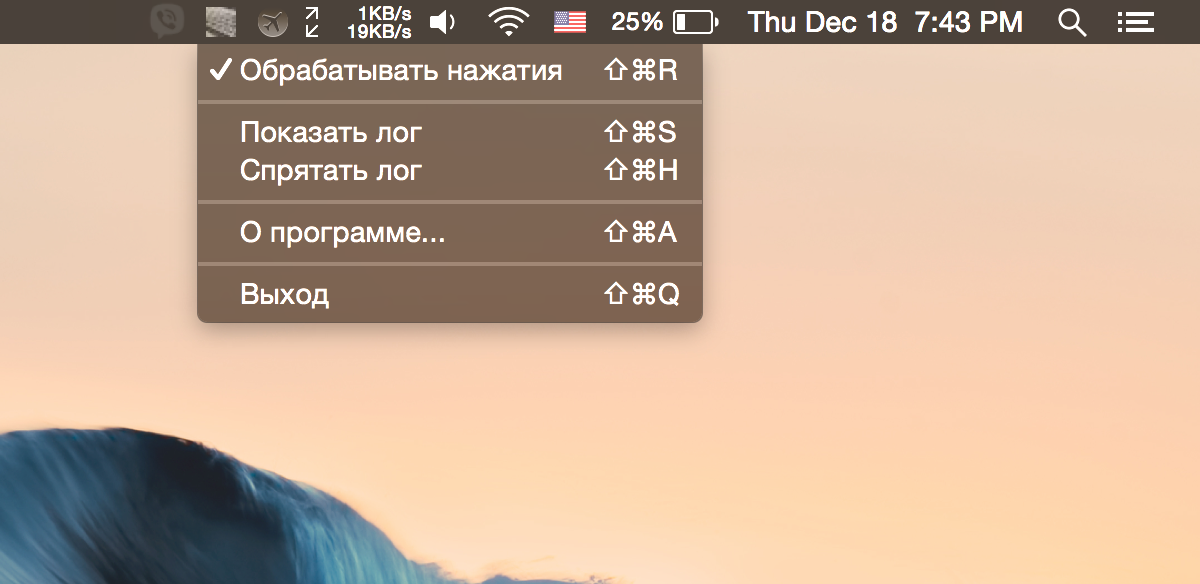
\includegraphics[width=130mm]{pic/statusbar.png}
  \caption{Меню приложения, доступное пользователю}
  \label{pic:statusbar}
\end{figure}

\begin{figure}[h!]
  \centering
  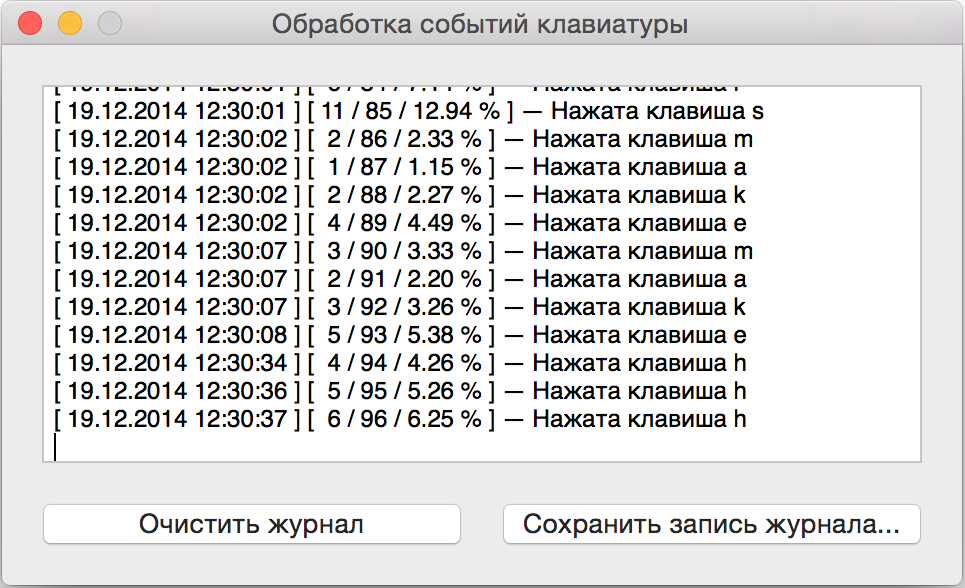
\includegraphics[width=130mm]{pic/log_window_in_work.png}
  \caption{Журнал с записями о нажатых клавишах}
  \label{pic:log_window_in_work}
\end{figure}

\newpage

Нажав кнопку <<Сохранить запись журнала...>> откроется вспомогательное окно,
в котором пользователю потребуется выбрать место для сохранения файла журнала
и имя этого журнала. Процесс сохранения журнала с записями о нажатых клавишах
на клавиатуре представлен на рисунке~\ref{pic:save_process}.

\begin{figure}[h!]
  \centering
  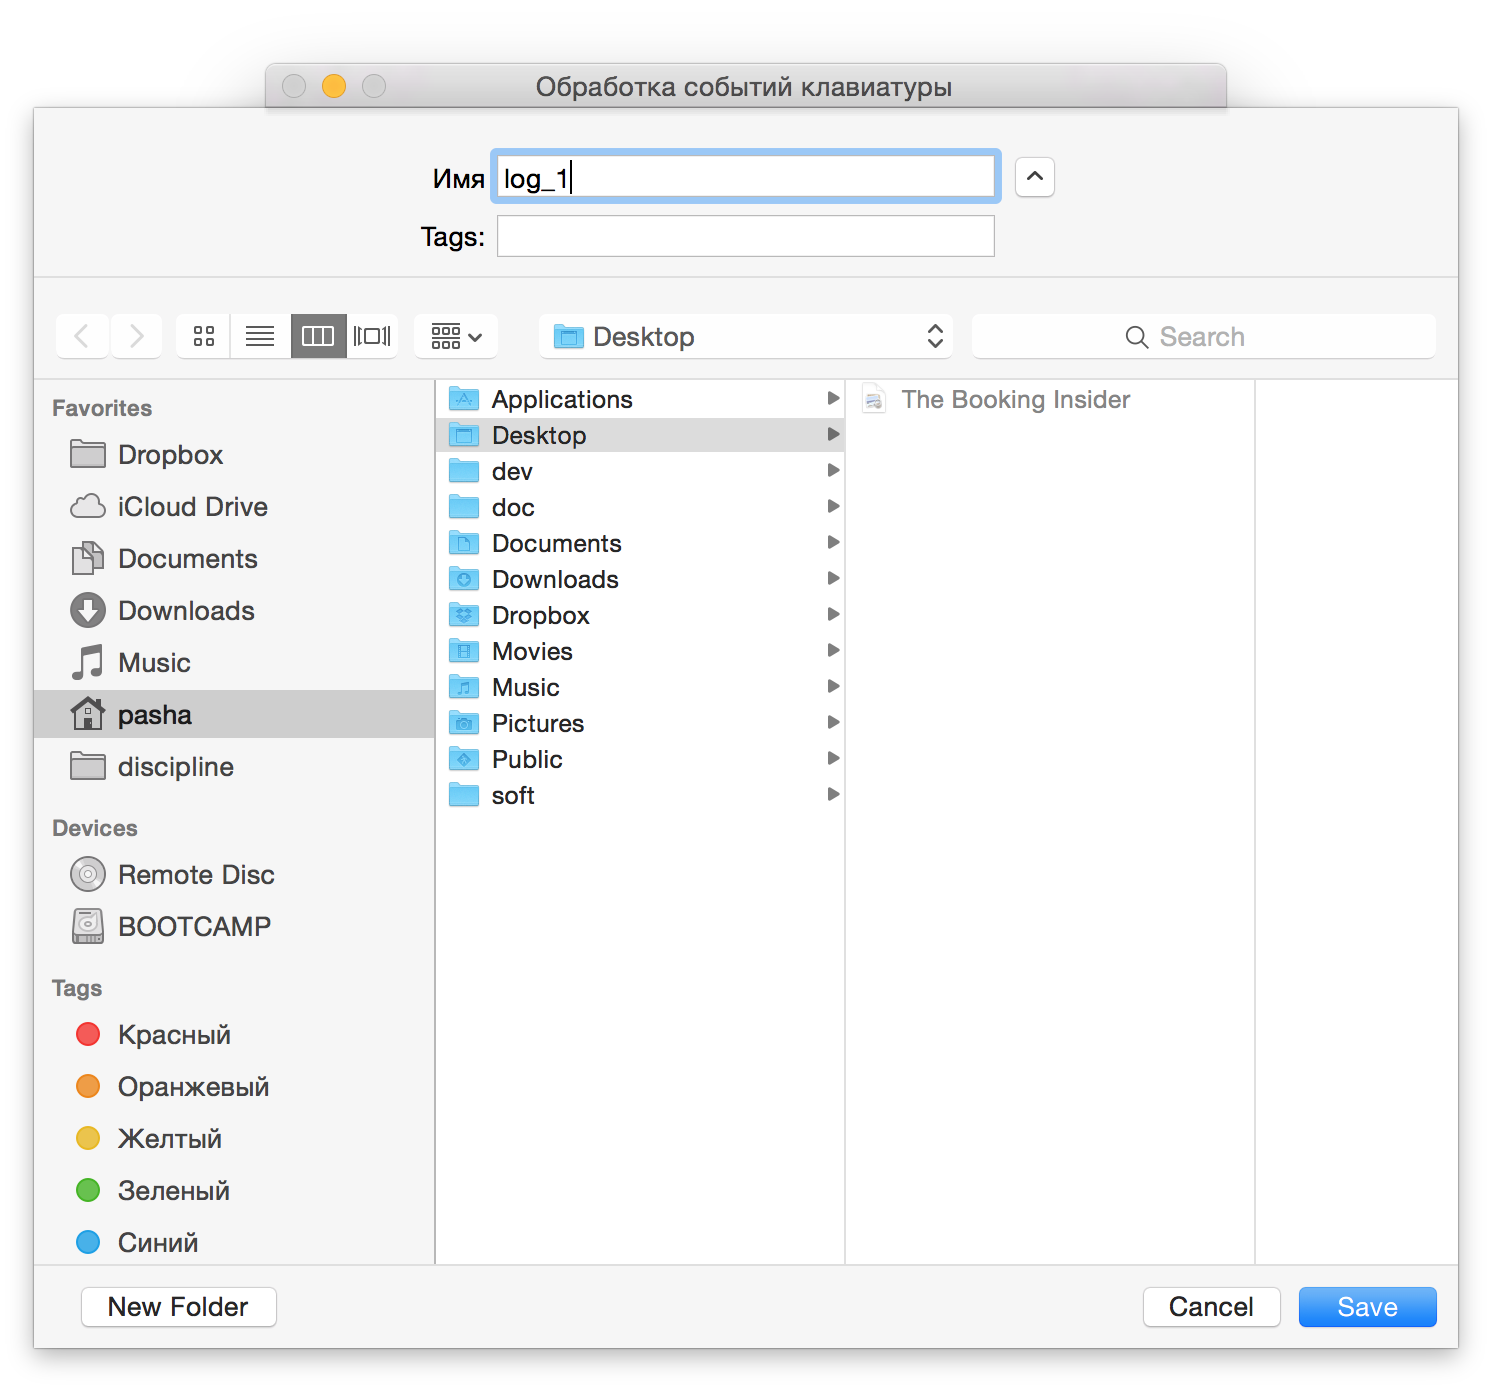
\includegraphics[width=130mm]{pic/save_process.png}
  \caption{Сохранение журнала с записями \\ о нажатых клавишах}
  \label{pic:save_process}
\end{figure}

\pagebreak
